\documentclass[11pt, a4paper]{article}

\usepackage[T1]{fontenc}
\usepackage[utf8]{inputenc}
\usepackage[norsk]{babel}
\usepackage{amsmath, amssymb, amsfonts, amsthm}
\usepackage{bbm}
\usepackage{graphicx}
\usepackage{verbatim}
\usepackage{caption}
\usepackage{subcaption}
\usepackage{subfig}
\usepackage{float}

\newcommand{\vb}{\mathbf}

\addto{\cationsnorsk}{
  \renewcommand{\contentsname}
    {Innhald}
}

\addto{\cationsnorsk}{
  \renewcommand{\abstractname}
    {Samandrag}
}

\begin{document}

\begin{titlepage}

  \title{\normalsize FYS1120 Elektromagnetisme\\
    \vspace{10mm}
    \huge Labøving\\
    \vspace{10mm}
    \normalsize{\bf Hall-effekt.}}

  \author{Øyvind Sigmundson Schøyen, Kristian Tuv og Hilde Solesvik Skeie}

\end{titlepage}

\maketitle

\newpage
  \tableofcontents
\newpage

\section*{Oppgåve 1}
\addcontentsline{toc}{section}{Oppgåve 1}

  \subsection*{PRELAB-Oppgåve 1}
  \addcontentsline{toc}{subsection}{PRELAB-Oppgåve 1}
    Me vil lage eit program som tek imot datapunkter $x$ og $y$ og gjer oss eit plott over punkta mot eit polynom som interpolerer dei. \\ \\
    Eg har nytta Python kor metodane $\texttt{polyval}$ og $\texttt{polyfit}$ ligg i numpy-biblioteket. Me er då interesserte i eit program som les datapunkt frå ei fil
    og prøver å finne eit polynom som gjer oss ein god modell.
    \verbatiminput{\string~/Documents/3.Semester/FYS1120/Lab/Hall-effekt/src/PRELABOppgave1.py}

  \subsection*{Oppgåve 1.1}
  \addcontentsline{toc}{subsection}{Oppgåve 1.1}
    Me vil bestemme retningen til $\vb{B}$ og retningen til straumen gjennom prøven (p-Ge). Me lager ei skisse som viser Hall-spenninga sin polaritet.
    Deretter måler me Hall-spenninga $V_{H}$ som ein funksjon av $B$ ved konstant $I$. \\ \\
    Me byrjar med å sette opp måleinstrumenta som består av to straumforsyningar, eit amperemeter, eit voltmeter og ein spole for å lage eit magnetfelt.
    Me stiller på straumforsyninga til me får $I \approx 24.132$ A gjennom komponenten (p-Ge). Då stiller me på potmeteret til me måler $V = 0$ gjennom komponenten.
    No målar me spenninga over komponenten når me held han i magnetfeltet mellom spolane for forskjellige straumverdiar og $B$-felt. Retningen til $B$-feltet finner me ved 
    høgrehandsregelen. % Legg ved teikning.
    Hall-spenningas polaritet finn me og ved høgrehandsregelen. Me peiker i retninga til driftshastigheta med peikefingeren. Resten av fingrane peiker me i retning av $B$-feltet.
    Då gjer tommelen oss retninga på krafta og me finn ut kor ladninga legg seg. % Legg ved teikning.
    \begin{center}
      \begin{tabular}{|l|l||l|}
        \hline
        $I$ & $B$ & $V$ \\
        \hline
        0.0 A & 6 mT & 1.4 mV \\
        0.2 A & 42 mT & 6.14 mV \\
        0.4 A & 74 mT & 11.47 mV \\
        0.6 A & 108 mT & 16.7 mV \\
        0.8 A & 142 mT & 22.0 mV \\
        1.0 A & 175 mT & 27.24 mV \\
        \hline
      \end{tabular}
    \end{center}

  \subsection*{Oppgåve 1.2}
  \addcontentsline{toc}{subsection}{Oppgåve 1.2}
    Her vil me rekne ut $R_{H}$ og $N$ gjeve ved
    \begin{align*}
      R_{H} = \frac{V_{H}d}{IB} = \frac{1}{Nq} \qquad \Rightarrow \qquad N = \frac{1}{R_{H}q}.
    \end{align*}
    Me vil no måle spenningsfallet over Ge-prøva i straumretninga. Dette nyttar me for å finne driftshastigheta $v$ som me vil samanlikne med hastigheta til eit elektron som 
    starter i ro i eit vakuum kor elektronet er utsatt for $E$-feltet som me får frå spenningskjelda over heila lengda $L$. \\ \\
    
    Me finner Hall-koeffisienten ved å ta endring i spenninga over endring i magnetfeltet. Då får me resultata under.
    \begin{center}
      \begin{tabular}{|l|l||l|}
        \hline
        $\Delta V$ & $\Delta B$ & $R_{H}$ \\
        \hline
        \input{\string~/Documents/3.Semester/FYS1120/Lab/Hall-effekt/src/RH_utskrift.txt}
        \hline
      \end{tabular}
    \end{center}

    Ladninga $q \approx 1.6\times10^{-19}C$ som er elementærladninga til eit proton.
    \begin{center}
      \begin{tabular}{|l||l|}
        \hline
        $R_{H}$ & $N$ \\
        \hline
        \input{\string~/Documents/3.Semester/FYS1120/Lab/Hall-effekt/src/N_utskrift.txt}
        \hline
      \end{tabular}
    \end{center}

    For å finne gjennomsnittshastigheta former me om uttrykket for $V_{H}$. Då får me
    \begin{align*}
      V_{H} = bvB = \frac{IB}{Nqd} \qquad \Rightarrow \qquad v = \frac{I}{Nqdb}.
    \end{align*}
    Me tek gjennomsnittet frå dei forskjellige verdiane av $N$. Då får me resultatet under.
    \begin{align*}
      \input{\string~/Documents/3.Semester/FYS1120/Lab/Hall-effekt/src/v_mean_utskrift.txt}
    \end{align*}
    Me finner hastigheta til eit elektron i vakuum ved å sjå på energi. Me vil sjå på omforminga frå potensiellenergi frå potensialet gonga med ladninga $q$ til kinetisk energi.
    \begin{align*}
      U = qV = \frac{1}{2}mv_e^2 \qquad \Rightarrow \qquad v_e = \sqrt{\frac{2qV}{m}}.
    \end{align*}
    Me finner potensialet $V$ ved å måle spenningsfallet over komponenten. Me koplar voltmeteret langs straumretninga. Då finner me $V \approx 1$ V.
    \begin{align*}
      \input{\string~/Documents/3.Semester/FYS1120/Lab/Hall-effekt/src/v_e_utskrift.txt}
    \end{align*}


  \subsection*{Oppgåve 1.3 og oppgåve 1.4}
  \addcontentsline{toc}{subsection}{Oppgåve 1.3 og oppgåve 1.4}
    Me gjentek stega frå $\textbf{Oppgåve 1.1}$ og $\textbf{Oppgåve 1.2}$ men for n-Ge. \\ \\
    Når me no skal finne Hall-spenningas polaritet må me nytte venstre handa til å finne retninga. Dette då me no arbeidar med negative ladningar.
    \begin{center}
      \begin{tabular}{|l|l||l|}
        \hline
        $I$ & $B$ & $V$ \\
        \hline
        0.0 A & 8 mT & -2 mV \\
        0.1 A & 33 mT & -5.34 mV \\
        0.2 A & 56 mT & -6.84 mV \\
        0.3 A & 81 mT & -12.4 mV \\
        0.4 A & 101 mT & -15.84 mV \\
        0.5 A & 121 mT & -18.67 mV \\
        \hline
      \end{tabular}
    \end{center}
    Me finner $R_{H}$, $N$ og gjennomsnittelig driftshastighet $v$.

    \begin{center}
      \begin{tabular}{|l|l||l|}
        \hline
        $\Delta V$ & $\Delta B$ & $R_{H}$ \\
        \hline
        \input{\string~/Documents/3.Semester/FYS1120/Lab/Hall-effekt/src/RH_utskrift2.txt}
        \hline
      \end{tabular}
    \end{center}

    \begin{center}
      \begin{tabular}{|l||l|}
        \hline
        $R_{H}$ & $N$ \\
        \hline
        \input{\string~/Documents/3.Semester/FYS1120/Lab/Hall-effekt/src/N_utskrift2.txt}
        \hline
      \end{tabular}
    \end{center}

    \begin{align*}
      \input{\string~/Documents/3.Semester/FYS1120/Lab/Hall-effekt/src/v_mean_utskrift2.txt}
    \end{align*}

  \subsection*{Oppgåve 1.5}
  \addcontentsline{toc}{subsection}{Oppgåve 1.5}
    Det kjem fram frå forteikna at me i p-Ge jobbar med positive ladningar og i n-Ge jobbar med negative ladningar. Storleiken på $R_{H}$ er annleis for n-Ge og p-Ge.
    Den er mykje mindre for n-Ge'en. Me ser og at $N$ er mykje større. Dette kjem fra fordi me har større konsentrasjon av elektron per areal då me har negativ ladning. For
    p-Ge'en vil me ha hol kor det manglar elektron.


\newpage


\section*{Oppgåve 2}
\addcontentsline{toc}{section}{Oppgåve 2}

  \subsection*{PRELAB-Oppgåve 2.1}
  \addcontentsline{toc}{subsection}{PRELAB-Oppgåve 2.1}
    Me vil vise at straumtettheten $j$ er identisk med magnetiseringa $M$. \\ \\
    Det enklaste er å sjå på einingane til $j$ og $M$. Me får
    \begin{align*}
      j = \frac{dI}{dx} = \frac{I}{t} \sim \frac{\text{A}}{\text{m}},
    \end{align*}
    kor straumen $I$ er målt i Ampere og distansen $dx$ er gjeve i meter. $M$ er gjeve som magnetisk moment per volumeining. Då får me
    \begin{align*}
      M = \frac{\vb{\mu}}{V} = \frac{IA}{V} = \frac{I\pi a^2}{\pi a^2t} = \frac{I}{t} \sim \frac{\text{A}\text{m}^2}{\text{m}^3} = \frac{\text{A}}{{m}}.
    \end{align*}
    I tillegg til å få dei same einingane veit me at me jobber med dei same ``metrane''.

  \subsection*{PRELAB-Oppgåve 2.2}
  \addcontentsline{toc}{subsection}{PRELAB-Oppgåve 2.2}
    Vis at me ved å integrere opp overflatestraumen kan skrive magnetfeltet som
    \begin{align*}
      B_x(h) = \frac{\mu_0}{2}j\left[ \frac{h + t}{\sqrt{(h + t)^2 + a^2}} - \frac{h}{\sqrt{h^2 + a^2}} \right].
    \end{align*} \\ \\
    Me set inn uttrykket for straumen $I$ i uttrykket for $B_x(x)$.
    \begin{align*}
      j = \frac{dI}{dx} \qquad \Rightarrow \qquad I = j\ dx
    \end{align*}
    Då får me 
    \begin{align*}
      B_x &= \frac{\mu_0}{2}I \frac{a^2}{(x^2 + a^2)^{3/2}} \\
      &= \frac{\mu_0}{2}j\frac{a^2}{(x^2 + a^2)^{3/2}}\ dx \\
      &= \frac{\mu_0}{2}ja^2\int_h^{h + t}\frac{dx}{(x^2 + a^2)^{3/2}} \\
      &= \frac{\mu_0}{2}ja^2\left[ \frac{x}{a^2\sqrt{x^2 + a^2}} \right]_h^{h + t} \\
      &= \frac{\mu_0}{2}j\left[ \frac{h + t}{\sqrt{(h + t)^2 + a^2}} - \frac{h}{\sqrt{h^2 + a^2}} \right].
    \end{align*}

  \subsection*{PRELAB-Oppgåve 2.3}
  \addcontentsline{toc}{subsection}{PRELAB-Oppgåve 2.3}
    I denne oppgåven vil me teste programmet frå $\textbf{PRELAB-Oppgåve 1}$ med likninga frå $\textbf{PRELAB-Oppgåve 2.2}$.
    Me vil nytte 5-6 punkter for $t = 35$ mm og $a = 20$ mm. \\ \\
    Fyrst finner me vakuum permeabiliteten $\mu_0 = 4\pi \times 10^{-7}$ Vs/(Am) frå læreboka. For å finne $j$ nyttar me resultatet frå $\textbf{PRELAB-Oppgåve 2.1}$.
    \begin{align*}
      j = M = \frac{IA}{V} = \frac{I\pi a^2}{\pi a^2t} = \frac{I}{t}.
    \end{align*}
    kor straumen $I$ vert valgt til $I = 0.1$ A. Me får då resultatet
    \begin{figure}[H]
      \centering
      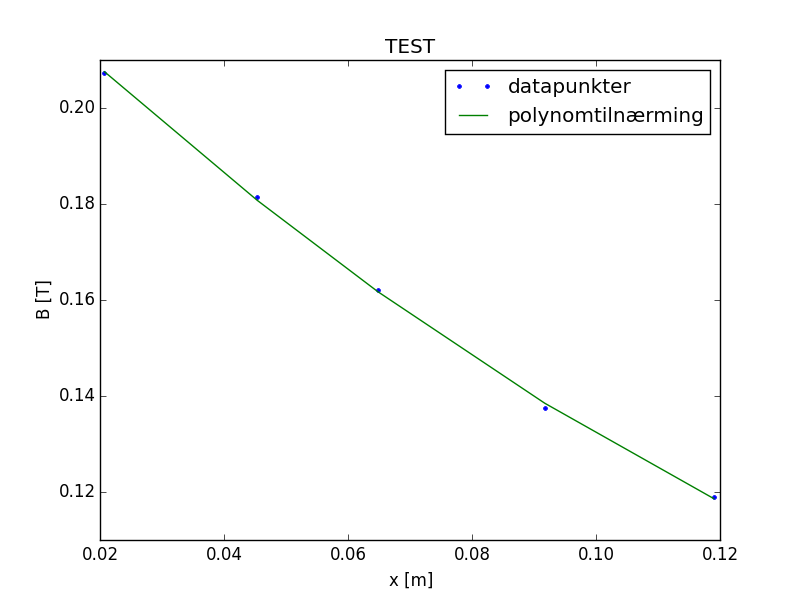
\includegraphics[width=400px]{\string~/Documents/3.Semester/FYS1120/Lab/Hall-effekt/src/PRELAB3.png}
      \caption{Her kan me sjå korleis polyfit prøver å tilpasse eit polynom til 6 punkter. Desverre vil det for så få punkter vere vanskeleg å gje eit nøyaktig resultat.}
    \end{figure}
    og utskrifta;
    \verbatiminput{\string~/Documents/3.Semester/FYS1120/Lab/Hall-effekt/src/Oppgave3.txt}
    Programmet $\texttt{PRELABOppgave3.py}$ er gjeve ved;
    \verbatiminput{\string~/Documents/3.Semester/FYS1120/Lab/Hall-effekt/src/PRELABOppgave3.py}

  \subsection*{PRELAB-Oppgåve 2.4}
  \addcontentsline{toc}{subsection}{PRELAB-Oppgåve 2.4}
    Me er interesserte i å sjå på $B$-feltet i topp-flata av magneten og når $t \to \infty$. Då lurer me og på kva $B$-feltet midt i sylinderen vert for noko. \\ \\
    Me startar med å sette inn $h = 0$ for å finne $B$-feltet i topp-flata. Me får
    \begin{align*}
      B_x(0) &= \frac{\mu_0}{2}j\left[ \frac{t}{\sqrt{t^2 + a^2}} - 0 \right] \\
      &= \frac{\mu_0}{2}\frac{tj}{\sqrt{t^2 a^2}}.
    \end{align*}
    For $t \to \infty$ får me
    \begin{align*}
      \lim_{t \to \infty} B_x(h) &= \lim_{t \to \infty} \frac{\mu_0}{2}j\underbrace{\left[ \frac{t}{\sqrt{t^2}} - \frac{h}{\sqrt{h^2 + a^2}} \right]}_{\approx 1} \\
      &= \frac{\mu_0}{2}j.
    \end{align*}
    Midt i sylinderen har me at $h = -\frac{t}{2}$ det gjer oss
    \begin{align*}
      B_x(-\frac{t}{2}) &= \frac{\mu_0}{2}j\left[ \frac{t}{2\sqrt{(t/2)^2 + a^2}} + \frac{t}{2\sqrt{(-t/2)^2 + a^2}} \right] \\
      &= \frac{\mu_0}{2}\frac{t}{\sqrt{(t/2)^2 + a^2}}.
    \end{align*}



  \subsection*{Oppgåve 2.1}
  \addcontentsline{toc}{subsection}{Oppgåve 2.1}
    Me vil måle $a$, $t$ og $B_{x}(h)$ i eit utvalg av avstandar frå overflata. Deretter vil me plotte i MATLAB for å samanlikna med den interpolerte funksjonen. \\ \\
    Måleverdiane våre vert
    \begin{center}
      \begin{tabular}{|l|l|}
        \hline
        $h$ & $B_{x}(h)$ \\
        \hline
        0 cm & 278 mT \\
        1 cm & 111.6 mT \\
        2 cm & 50.9 mT \\
        3 cm & 24.9 mT \\
        4 cm & 14.6 mT \\
        5 cm & 10 mT \\
        6 cm & 7.1 mT \\
        7 cm & 5.2 mT \\
        8 cm & 4 mT \\
        9 cm & 3.1 mT \\
        10 cm & 2.7 mT \\
        \hline
      \end{tabular}
    \end{center}

    MATLAB gjer oss grafen;
    \begin{figure}[H]
      \centering
      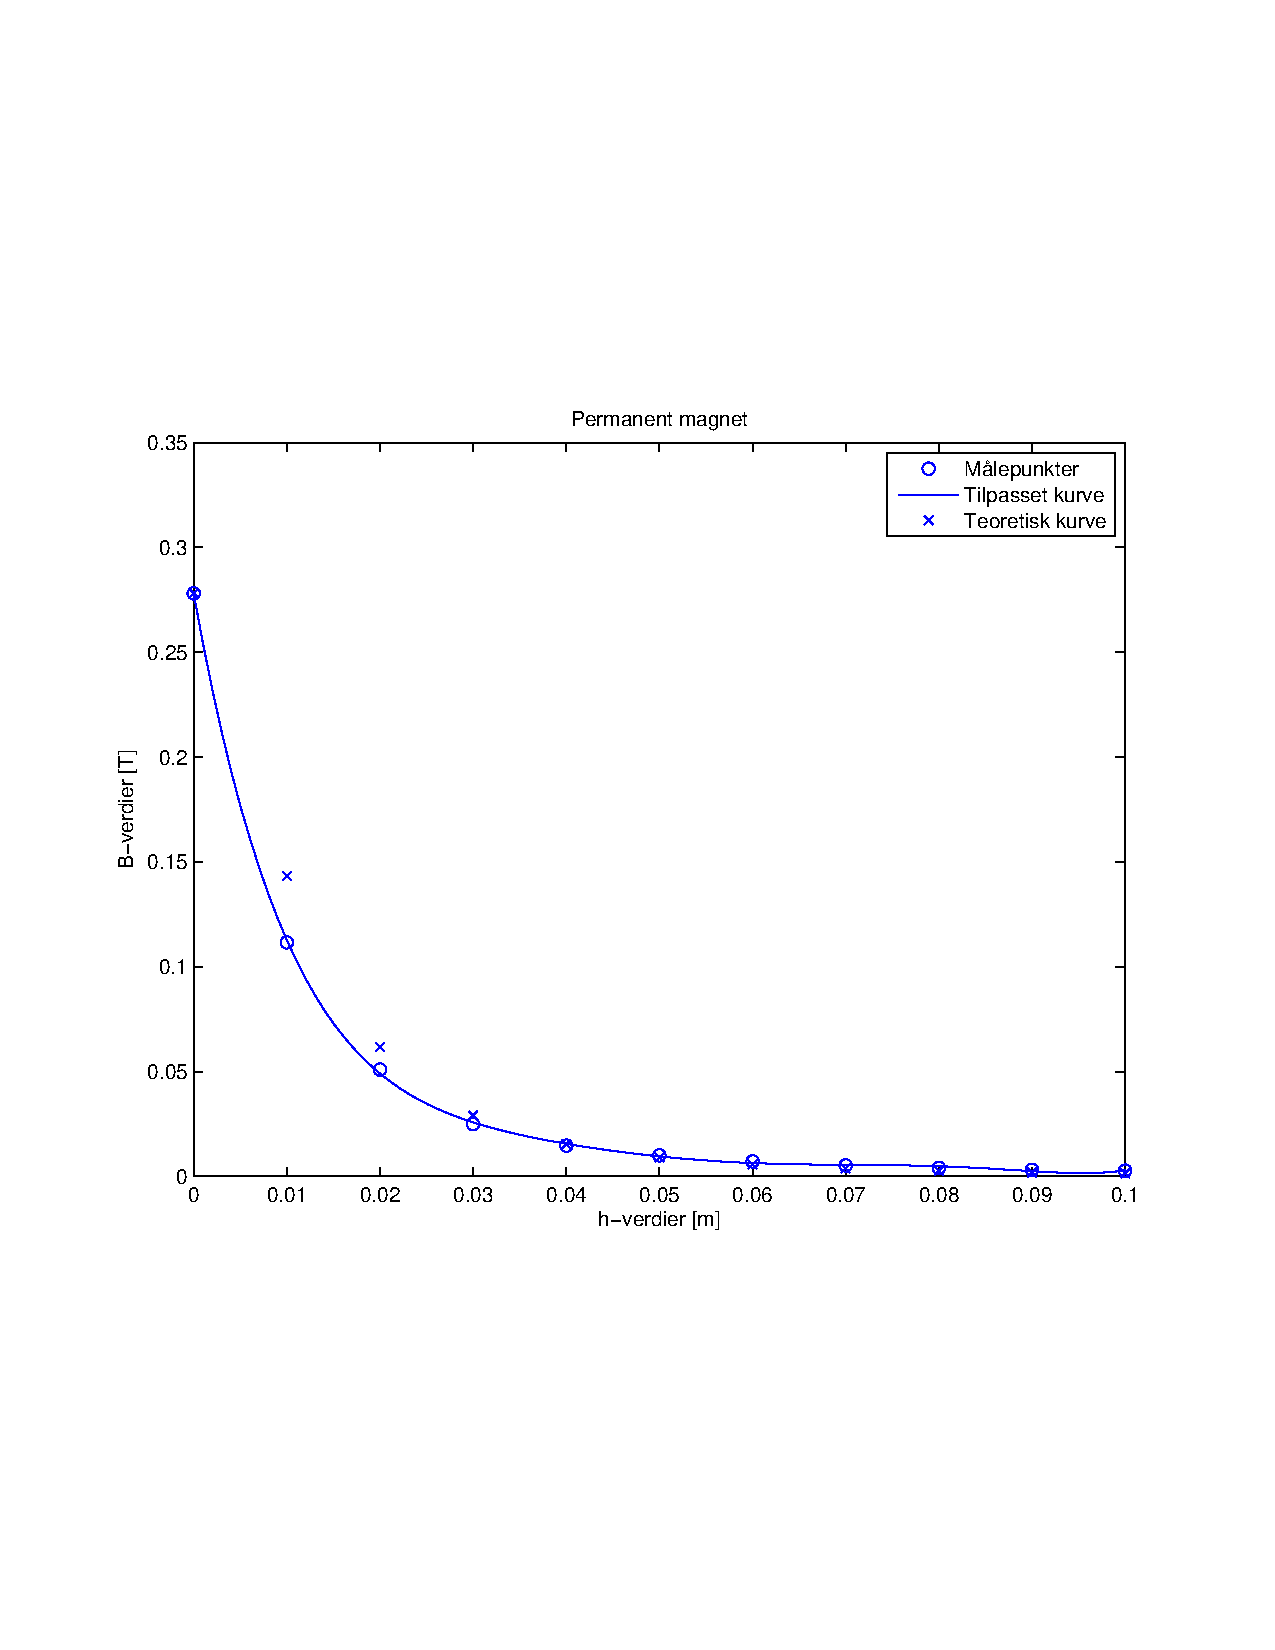
\includegraphics[width=400px]{Oppgave21.pdf}
      \caption{Modellen stemmer bra med målepunkta.}
    \end{figure}

    Denne får me frå programmet
    \verbatiminput{Oppgave2_1.m}

  \subsection*{Oppgåve 2.2}
  \addcontentsline{toc}{subsection}{Oppgåve 2.2}
    Me vil no finne verdien for $\mu_0 j$. \\ \\
    Me former om likninga for $B_{x}(h)$ slik at me får
    \begin{align*}
      \frac{2B}{z} = \mu_0j,
    \end{align*}
    kor
    \begin{align*}
      z = \frac{h + t}{\sqrt{(h + t)^2 + a^2}} - \frac{h}{\sqrt{h^2 + a^2}}.
    \end{align*}
    Me har valgt $h = 0.0$ m og $B = 278$ mT.
    Då finner me
    \begin{align*}
      \mu_0 j = 1.13 \text{ T}.
    \end{align*}
    Det stemmer overens med magnetar laga av NdFeB som har ein remanent induksjon på ca $1.2$ T.

\newpage

\section*{Oppgåve 3}
\addcontentsline{toc}{section}{Oppgåve 3}
  Her vil me måle $B_{x}(h)$ for ein sylindrisk elektromagnet i forskjellige høgdar frå overflata og eit punkt inne i sylinderen. Me lager ein graf i MATLAB som viser punkta og
  samanliknar med formelen for $B_{x}(h)$. \\ \\
  Me fekk då måleverdiane
  \begin{center}
    \begin{tabular}{|l|l|}
      \hline
      $h$ & $B_{x}(h)$ \\
      \hline
      0 cm & 2.8 mT \\
      1 cm & 2.0 mT \\
      2 cm & 1.5 mT \\
      3 cm & 1.1 mT \\
      4 cm & 0.9 mT \\
      5 cm & 0.6 mT \\
      6 cm & 0.4 mT \\
      7 cm & 0.3 mT \\
      8 cm & 0.2 mT \\
      9 cm & 0.1 mT \\
      10 cm & 0.0 mT \\
      \hline
    \end{tabular}
  \end{center}
  over overflata og inne i sylinderen vert det $B = 5.3$ mT. Uttrykket for $j$ finner me då ved
  \begin{align*}
    j = \frac{N\mu}{V} = \frac{NIA}{V} = \frac{NI}{t},
  \end{align*}
  kor $t$ er lengda og $N$ er antal vindingar.
  Dette fant me blant annet frå $\textbf{PRELAB-Oppgåve 2.1}$.

  MATLAB gjer oss då grafen
  \begin{figure}[H]
    \centering
    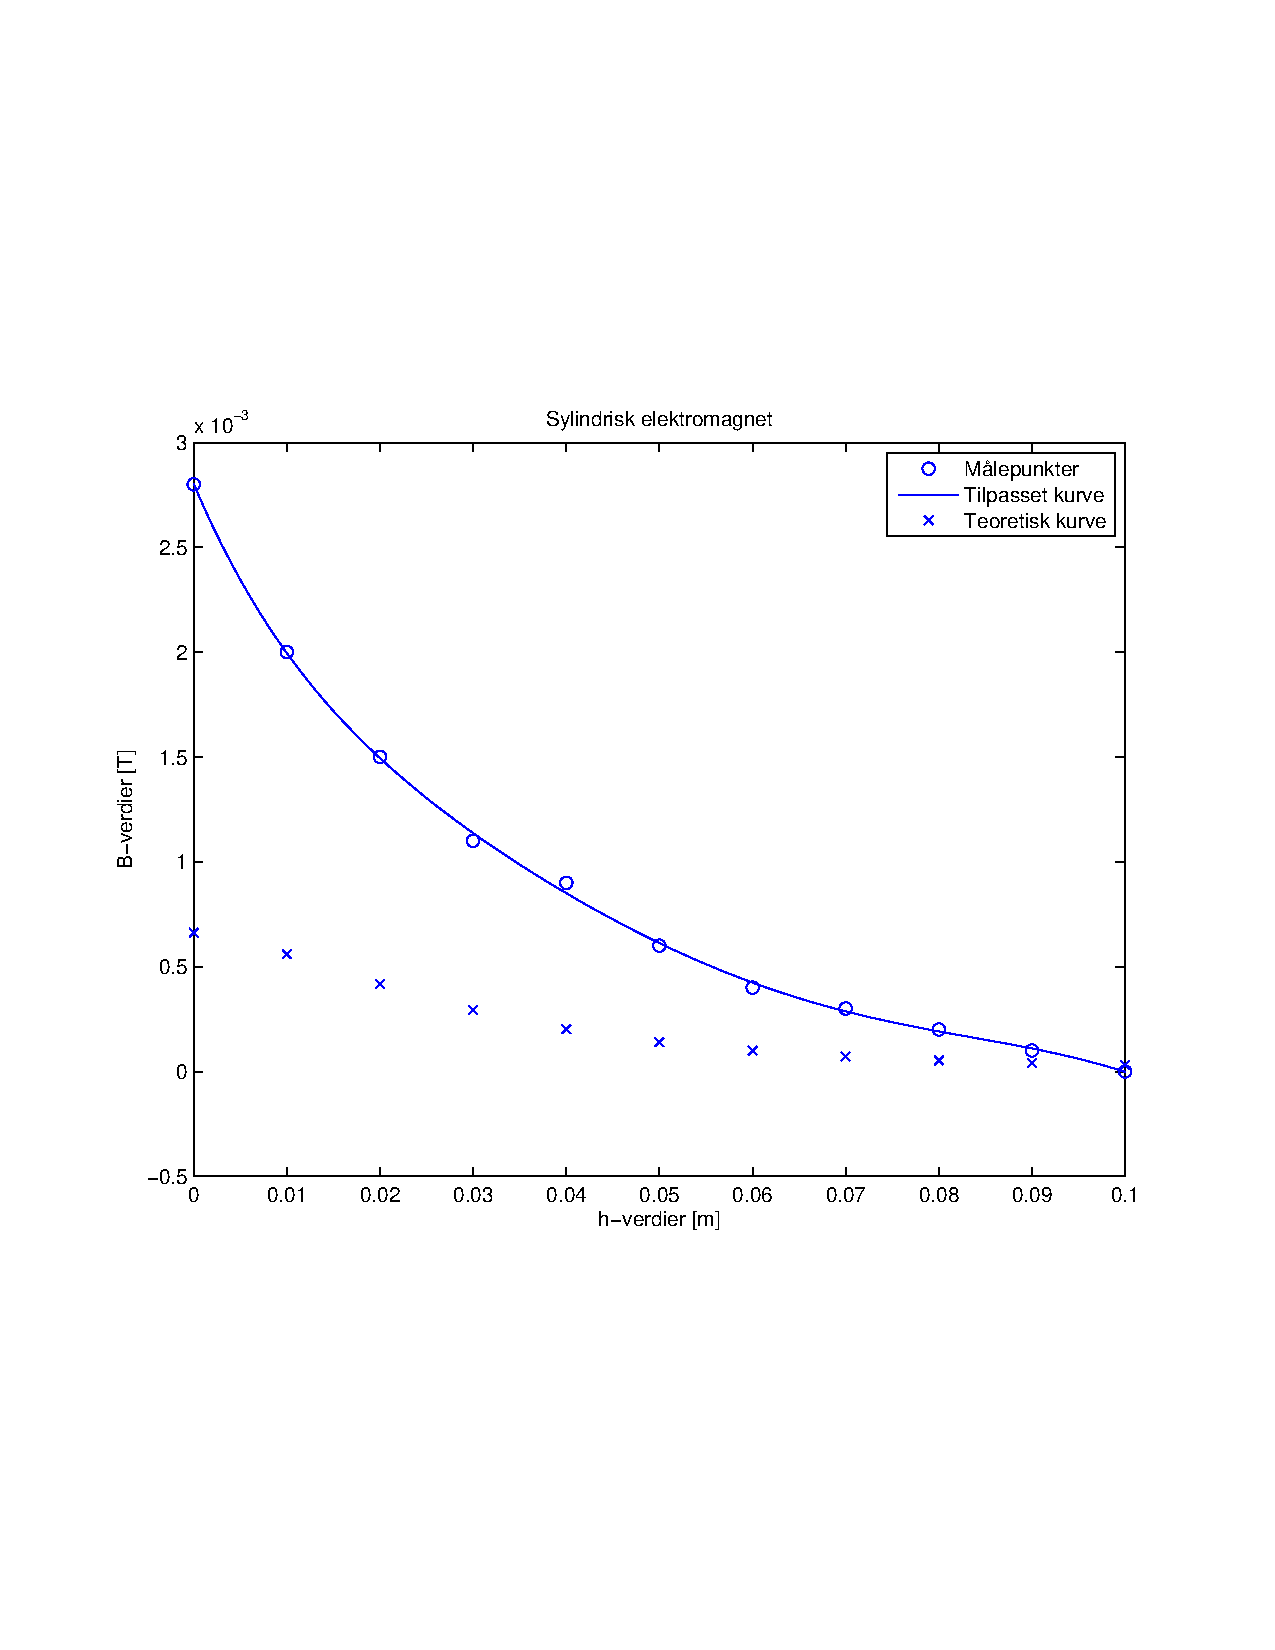
\includegraphics[width=400px]{Oppgave3.pdf}
    \caption{Denne grafen er feil, men me fant ikkje feilen.}
  \end{figure}

  Programmet er skrive
  \verbatiminput{Oppgave3.m}







\end{document}
